\documentclass{article}
\usepackage{vub}
\usepackage[utf8]{inputenc}
\usepackage[dutch]{babel}
\usepackage{xcolor}
\usepackage{array}
\usepackage{graphicx}
\usepackage{tabularx}
\title{Programmeerproject 2}
\subtitle{Documentatie fase 3}
\definecolor{myblueish}{rgb}{0.36, 0.54, 0.66}
\faculty{Sciences and Bio-Engineering Sciences}
\author{Gérard Lichtert\\
        \textcolor{blue}{gerard.Lichtert@vub.be}\\
        \textcolor{myblueish}{0557513}}
\date{\today}
\begin{document}
\maketitle
\tableofcontents
\pagebreak
\section{Inleiding}
Dit document bevat het verslag van fase 3 van het vak "Programmeerproject 2". Het behandelt 
de eerste functionele vereisten en de 3 uigebreide vereisten. 
Vervolgens zal het over de gebruikte datastructuren gaan en het afhankelijkheids diagram. 
Deze datastructuren zullen er voor zorgen dat alle functionaliteiten werken en vanuit 
de GUI aangeroepen kunnen worden. Verder staat in dit verslag een beschrijving van de API tussen
de infrabel- en NMBS-component, de planning en het logboek. 
\section{Functionele vereisten}
In dit verslag worden de functionele vereisten per fase besproken. In de eerste fase werd de 
GUI gemaakt alsook de command and control. De code van de command en control moeten we zelf
niet schrijven maar de code die de hardware aanstuurt wel. De code moet locomotieven kunnen laten
starten en stoppen, hun snelheid en rijrichting aflezen en veranderen. Verder moeten we ook de 
de stand van de wissels kunnen uitlezen en verzetten. Via de detectieblokkken detecteren we waar 
een trein zich bevindt. \\
De GUI laat de eindgebruiker de toestand van het spoornetwerk en de locomotieven zien. Het laat 
ook interactie toe met de wissels en locomotieven. \\
In de tweede fase was het de bedoeling dat we de eerste twee uitgebreide vereisten implementeren. Voor dit project werd 
gekozen voor botsingpreventie aan de hand van een reservatie en bezettingsysteem. Dit zal ervoor zorgen dat een trein zijn snelheid 
op nul gezet wordt als het pad dat die gaat afleggen al gereserveerd of bezet is. Aangezien de stand van de wissels op eender welk moment gewijzigd kan worden, worden
er veel spoorsegmenten gereserveerd tot de aanliggende detectieblokken. Dit is wel met de voorwaarde dat ze op het pad zijn van de richting van de trein. Een andere
uitgebreide vereiste waar voor gekozen werd is het automatisch trajectbeheer. De manier waarop dit geimplementeerd is dat de eindbestemming ingevoerd wordt en het pad berekend
word. Dit wordt slechts gedaan als de trein detecteerbaar is. Anders zal het pad nog eens herberekend worden wanneer die detecteerbaar is. Er wordt bij het trajectbeheer
ook rekening gehouden met het reservatiesysteem om botsingen te voorkomen. \\
In de 3e fase is het de bedoeling dat we de laatste uitgebreide vereiste implementeren. Bij dit project is dit de Raspberry Pi vereiste. Dit houdt in dat het mogelijk
moet zijn om infrabel te runnen op de Raspberry Pi en NMBS op de computer. Dit wordt behaald door het externe IP adres (of lokaal) mee te geven bij het aanmaken van het NMBS object.
\pagebreak
\section{ADT's}
\subsection{Track ADT}
Het track ADT houdt bij welke spoorsegmenten verbonden zijn. Het houdt ook bij of het spoorsegment al dan niet
gereserveerd is. De reservatiestand kan ook aangepast worden. 
\begin{table}[h!]
        \centering
        \begin{tabular}{|p{2.9cm}|p{4cm}|p{6.1cm}|}
                \hline
                \multicolumn{1}{|>{\centering\arraybackslash}p{2.9cm}|}{\textbf{Naam}} 
                & \multicolumn{1}{>{\centering\arraybackslash}p{4cm}|}{\textbf{Signatuur}} 
                   & \multicolumn{1}{>{\centering\arraybackslash}p{6.1cm}|}{\textbf{Beschrijving}}\\
                \hline
                new & (symbol, list $\rightarrow$ track\%) & Maakt een track object aan. Verwacht
                de ID van het spoorsegment en een lijst met de ID's van de verbonden spoorsegmenten.\\
                \hline
                get-track-id & (/ $\rightarrow$ symbol) & Geeft de ID van het spoorsegment terug.\\
                \hline
                track-links & (/ $\rightarrow$ vector) & Geeft de vector terug met de ID's van de verbonden spoorsegmenten.\\
                \hline
                set-links! & (list $\rightarrow$ /) & Verandert de verbonden spoorsegmenten.\\
                \hline
                links-map & ((symbol $\rightarrow$ any) $\rightarrow$ vector) & Voert een procedure uit op de ID's van de verbonden spoorsegmenten en geeft de opgespannen vector terug.\\
                \hline
                reserved? & (/ $\rightarrow$ symbol $\cup$ false) & Geeft de ID van de locomotief die het spoorsegment gereserveerd heeft of false.\\
                \hline
                reserve! & (symbol $\rightarrow$ /) & Verandert de reservatiestatus naar het meegegeven ID.\\
                \hline
                cancel-reservation! & (/ $\rightarrow$ /) & Zet het reservatiestatus op false\\
                \hline
                nr-of-links & (/ $\rightarrow$ integer) & Geeft het aantal verbonden spoorsegmenten terug\\     
                \hline
                track? & (/ $\rightarrow$ boolean) & Test of iets tot de track classe behoort.\\
                \hline
        \end{tabular}
        \caption{Signaturen van track\%}            
\end{table}
\subsubsection{Toelichting}
Het track ADT is eigenlijk een superclasse van de volgende ADT's. Dit is zodat de volgende ADT's de methoden erven van het track ADT. New maakt een nieuwe track ADT aan. 
Dit kan ook vervangen worden door (make-object track\% \textless \space argumenten \textgreater). $get-track-id$ dient om de ID op te vragen. $track-links$ dient om de vector met verbonden
spoorsegmenten op te vragen. $set-links!$ wijzigt de verbonden spoorsegmenten. $links-map$ voert een procedure uit op de vector-elementen. 
$reserved?$ geeft of de ID van het locomotief terug die het spoorsegment gereserveerd heeft of false. $cancel-reservation!$ zet de reservatiestand naar false. 
$nr-of-links$ geeft het aantal verbindingen terug. Classen zoals switch en detectieblokken zullen de methoden erven van deze classe. 
\subsection{Switch ADT}
Het switch ADT erft de methoden van het Track ADT. Het zal dus bovenop de onderstaande
methoden ook de methoden van het Track ADT bevatten. Het switch ADT houdt de 
stand van een wissel bij, welk spoorsegment verbonden is met de huidige stand en 
het staat toe om de stand te veranderen. \\
\begin{table}[h!]
        \centering
        \begin{tabular}{|p{2.9cm}|p{4cm}|p{6.1cm}|}
                \hline
                \multicolumn{1}{|>{\centering\arraybackslash}p{2.9cm}|}{\textbf{Naam}} 
                & \multicolumn{1}{>{\centering\arraybackslash}p{4cm}|}{\textbf{Signatuur}} 
                   & \multicolumn{1}{>{\centering\arraybackslash}p{6.1cm}|}{\textbf{Beschrijving}}\\
                \hline 
                new & (symbol, list $\rightarrow$ switch\%) & Maakt een nieuwe switch object aan\\
                \hline
                get-status & (/ $\rightarrow$ integer) & Geeft de stand van de wissel terug. \\
                \hline
                set-status! & (integer $\rightarrow$ integer) & Veranert de stand van de wissel.  \\
                \hline
                get-merge-track & (/ $\rightarrow$ symbol) & Geeft de ID van het spoorsegment die niet met de stand
                van de wissels verandert. \\
                \hline
                get-linked-track & (/ $\rightarrow$ symbol) & Geeft de ID van het spoorsegment die verbonden is met de stand
                van de wissel. \\
                \hline
                switch? & (any $\rightarrow$ boolean) & Test of iets tot de switch classe behoort. \\
        \end{tabular}
        \caption{Signaturen van switch\%}
\end{table}
\subsubsection{Toelichting}
Het switch ADT is een subclasse van het track ADT. Het kan dus dezelfde methoden gebruik als het track ADT. De extra
methoden zijn $new$ dat dezelfde argumenten verwacht als het track ADT (De ID van het spoorsegment en een lijst met de ID's van
de verbonden spoorsegmenten.) Let op!: Zet de ID op de juste index in de lijst. Als de stand van een wissel 1 is en het verbindt
met het spoorsegment 1-5, dan zou de lijst '(U-1 1-5 ... etc...) moeten zijn. Dit is zodat de interne index van de stand van de wissels analoog is aan
de stand van de wissels van de hardware. $get-status$ geeft de stand van de wissel terug als een nummer. 
$set-status!$ verandert de stand van de wissel naar het gegeven stand.
Zorg er wel voor dat de index correct overeenkomt omdat het afleest van de vector
die de verbonden spoorsegmenten bijhoudt. $get-merge-track$ geeft de ID van het spoorsegment die niet met de stand
van de wissel verandert. $get-linked-track$ geeft de ID terug van de huidige verbonden spoorsegment aan de hand van de stand
van de wissel. 
\subsection{Dblock ADT}
Het detection block ADT is een subclasse van het track ADT. Het erft dus net zoals
het switch ADT de methoden van het track ADT. Bovendien houdt het ook bij of dat 
er zich een locomotief op bevindt. 
\begin{table}[h!]
        \centering
        \begin{tabular}{|p{2.9cm}|p{4cm}|p{6.1cm}|}
                \hline
                \multicolumn{1}{|>{\centering\arraybackslash}p{2.9cm}|}{\textbf{Naam}} 
                & \multicolumn{1}{>{\centering\arraybackslash}p{4cm}|}{\textbf{Signatuur}} 
                   & \multicolumn{1}{>{\centering\arraybackslash}p{6.1cm}|}{\textbf{Beschrijving}}\\
                \hline 
                new & (symbol, list $\rightarrow$ dblock\%) & Maakt een nieuw detectie block object aan.\\
                \hline
                occupied? & (/ $\rightarrow$ symbol $\cup$ false) & Geeft ID van de locomotief terug die momenteel 
                de detectieblok bezet. \\
                \hline
                occupy! & (symbol $\rightarrow$ /) & Bezet de detectieblok met het gegeven ID.\\
                \hline
                vacant! & (/ $\rightarrow$ /) & Maakt de detectieblok vrij. \\
                \hline
                dblock? & (/ $\rightarrow$ boolean) & Test of ietst tot de detectieblok classe behoort.\\ 
                \hline
        \end{tabular}
        \caption{Signaturen van dblock\%}
\end{table}
\subsubsection{Toelichting}
De methoden die bruikbaar zijn voor het detectieblok ADT zijn de methoden die het ADT erft van het track ADT. 
Dit is ook niet zonder de hierboven genoemde methoden die het arsenaal vervullen. $new$ maakt een nieuwe
detectieblok object aan. Het verwacht dezelfde argumenten zoals $new$ van het track ADT. $occupied?$ geeft de ID van de locomotief die
het detectieblok bezet of false indien die niet bezet is. $occupy!$ bezet het detectieblok met het gegeven ID van een locomotief. 
$vacant!$ zal er voor zorgen dat het detectieblok terug vrij is. 
\subsection{Locomotive ADT}
Het locomotief ADT houdt de interne data van een locomotief bij zoals snelheid, richting, vorige locatie, huidige locatie, manuele modus,
het pad en de eindbestemming. Dit komt natuurlijk ook met methoden om ze te veranderen. 
Het pad en eindbestemming wordt gebruikt voor het automatisch trajectbeheer. 
\begin{table}[h!]
        \centering
        \begin{tabular}{|p{2.9cm}|p{4cm}|p{6.1cm}|}
                \hline
                \multicolumn{1}{|>{\centering\arraybackslash}p{2.9cm}|}{\textbf{Naam}} 
                & \multicolumn{1}{>{\centering\arraybackslash}p{4cm}|}{\textbf{Signatuur}} 
                   & \multicolumn{1}{>{\centering\arraybackslash}p{6.1cm}|}{\textbf{Beschrijving}}\\
                \hline 
                new & (symbol, symbol, symbol, symbol $\rightarrow$ locomotive\%) & Maakt een nieuw lovomotief object aan.\\
                \hline
                reserve! & (list $\rightarrow$ /) & Slaat een lijst van ID's van spoorsegmenten op die de locomotief gereserveerd heeft.\\
                \hline
                clear-reservations! & (/ $\rightarrow$ /) & Verwijdert de lijst van reservaties. \\
                \hline
                made-reservations? & (/ $\rightarrow$ list $\cup$ false) & Geeft een lijst van ID's van de gereserveerde spoorsegmenten terug.\\
                \hline
                manual-override & (boolean $\rightarrow$ /) & Wijzigt de reservatieprotocol van de locomotief.\\
                \hline
                manual? & (/ $\rightarrow$ boolean) & Geeft het reservatieprotocol terug van de locomotief. \\
                \hline
                get-loco-id & (/ $\rightarrow$ symbol) & Geeft de ID van de locomotief terug. \\
                \hline
                locomotive? & (/ $\rightarrow$ boolean) & Test of iets tot de locomotief classe behoort.\\
                \hline
        \end{tabular}
        \caption{Signaturen van locomotive\%}
\end{table}
\subsubsection{Toelichting}
$new$ maakt een nieuw locomotief object aan. Het neemt als eerste de ID van de locomotief, de richting van de locomotief, de huidige locatie en de vorige locatie. 
$reserve!$ verwacht een lijst van ID's van spoorsegmenten die de locomotief gereserveerd heeft. $clear-reservations!$ verwijdert de lijst van ID's van de gereserveerde
spoorsegmenten. De waarde hiervan verandert naar $false$. $made-reservations?$ geeft of de lijst terug van de van de ID's van de gereserveerde spoorsegmenten of $false$ indien de 
locomotief geen spoorsegmenten gereserveerd heeft.
$manual-override$ zal dienen om de status van de manier van het reservatiesysteem te veranderen. Wanneer de status $true$ is zal het de bezetting van een detectieblok negeren, 
dit zal vooral dienen om naar dichtbijzijnde detectieblokken te kunnen navigeren zonder rekening te houden met locomotieven die te dicht in de buurt zijn. De enige argumenten
die dus gebruikt kunnen worden hiervoor zijn dus ook de booleans. 
$manual?$ geeft de status van de manuele modus terug. Als laatste $get-loco-id$ geeft de ID terug van de locomotief. 
\subsection{Railway ADT}
Het railway ADT brengt de de spoor gerelateerde ADT's zoals het track ADT, switch ADT, het detectieblok ADT en het locomotief ADT samen. 
Zo houdt he railway ADT het volledig spoornetwerk samen. Het netwerk zelf wordt bewaard in een graaf. Het programma maakt hierdoor gebruik van de $graph$ library. 
Buiten een graaf van het spoornetwerk zelf bewaart het ook een graaf met detectieblokken met bogen naar die gedefinieerd zijn op vlak van bereikbaarheid. Er is bijvoorbeeld dus een boog tussen
detectieblok 1-4 en 1-1 omdat er een pad is van deze detectieblokken waarbij er geen andere detectieblok tussen zit en dat de trein niet van richting moet veranderen tussen deze detectieblokken (wel op de detectieblok zelf!). Op basis hiervan kunnen we dus trajecten berekenen. Hiervan en een speciale graaf die alleen de detectieblokken bevat. Dit is zodat we kunnen
navigeren en paden kunnen berekenen aan de hand van paden tussen detectieblokken. De methoden van het Railway ADT zullen voornamelijk zoek-functionaliteiten aanbieden. 
Een voorbeeld hiervan is als we een locomotief object willen aanspreken dan zal het dit eerst opzoeken in de hashmap waar het opgeslagen staat. Hetzelfde geldt voor het 
aanspreken van een track ADT en zijn subclassen. 
\begin{table}[h!]
        \centering
        \begin{tabular}{|p{2.9cm}|p{4cm}|p{6.1cm}|}
                \hline
                \multicolumn{1}{|>{\centering\arraybackslash}p{2.9cm}|}{\textbf{Naam}} 
                & \multicolumn{1}{>{\centering\arraybackslash}p{4cm}|}{\textbf{Signatuur}} 
                   & \multicolumn{1}{>{\centering\arraybackslash}p{6.1cm}|}{\textbf{Beschrijving}}\\
                \hline 
                new & (/ $\rightarrow$ railway\%) & Maakt een nieuw railway object aan.\\
                \hline
                get-list-of-tracks & (/ $\rightarrow$ list) & Geeft een lijst van terug van de hashmap van alle spoorsegmenten.\\
                \hline
                get-track & (/ $\rightarrow$ track $\cup$ dblock $\cup$ switch $\cup$ false) & Geeft het gezochte spoor object terug. \\
                \hline
                make-track & (symbol, list $\rightarrow$ track) & Maakt een track object aan.\\
                \hline
                make-switch & (symbol, list $\rightarrow$ switch) & Maakt een wissel object aan.\\
                \hline
                make-dblock & (symbol, list $\rightarrow$ dblock) & Maakt een detectieblok object aan. \\
                \hline
                add-track! & (track $\cup$ dblock $\cup$ switch $\rightarrow$ track $\cup$ dblock $\cup$ switch) & Voegt het spoor object toe aan het spoornetwerk.\\
                \hline
                remove-track! & (symbol $\rightarrow$ /) & Verwijdert het gezochte object uit het spoornetwerk. \\
                \hline
                update-track! & (symbol (track $\cup$ dblock $\cup$ switch $\rightarrow$ any) $\rightarrow$ /) & Voert de meegegeven procedure uit op het gezochte object. \\
                \hline
                for-each-track & ((track $\cup$ dblock $\cup$ switch $\rightarrow$ any) $\rightarrow$ any) & Voert een procedure uit op alle spoorsegmenten \\
                \hline
                for-each-link &  ((track $\cup$ dblock $\cup$ switch $\rightarrow$ any), symbol $\rightarrow$ vector) & Voert een procedure uit op de aanliggende spoorsegmenten van het gezochte spoorsegment.\\   
                \hline
                get-railway-graph & (/ $\rightarrow$ graph) & Geeft de graaf met het spoornetwerk terug.\\
                \hline
        \end{tabular}
        \caption{Signaturen van railway\%}
\end{table}
\begin{table}[h!]
        \centering
        \begin{tabular}{|p{2.9cm}|p{4cm}|p{6.1cm}|}
                \hline
                \multicolumn{1}{|>{\centering\arraybackslash}p{2.9cm}|}{\textbf{Naam}} 
                & \multicolumn{1}{>{\centering\arraybackslash}p{4cm}|}{\textbf{Signatuur}} 
                   & \multicolumn{1}{>{\centering\arraybackslash}p{6.1cm}|}{\textbf{Beschrijving}}\\
                \hline 
                get-dblock-graph & (/ $\rightarrow$ graph) & Geeft de graaf met alleen detectieblokken terug. \\
                \hline
                make-locomotive & (symbol, symbol, symbol, symbol $\rightarrow$ locomotive) & Maakt een locomotief object aan aan de hand van de gegeven
                ID, richting, huidige detectieblok en vorige detectieblok. \\
                \hline
                add-locomotive! & (locomotive $\rightarrow$ /) & Voegt een locomotief object toe aan het spoornetwerk.\\
                \hline
                remove-locomotive! & (symbol $\rightarrow$ /) & Verwijdert het gezochte locomotief object van het spoornetwerk. \\
                \hline
                update-locomotive! & (locomotive $\rightarrow$ /) & Verandert gegevens van een locomotief door het te vervangen met een nieuwe. \\
                \hline
                get-locomotive & (symbol $\rightarrow$ locomotive $\cup$ false) & Geeft het gezochte locomotief object terug of false indien deze niet bestaat. \\
                \hline
                for-each-loco & ((locomotive $\rightarrow$ any) $\rightarrow$ any) & Voert een procedure uit op alle locomotief objecten. \\
                \hline
                railway? & (any $\rightarrow$ boolean) & Geeft terug of iets tot de railway classe behoort. \\
                \hline
        \end{tabular}
        \caption{Vervolg van de signaturen van railway\%}
\end{table}
\subsubsection{Toelichting}
Niet alle methoden zullen besproken worden omdat sommige methoden zoals $make-switch$, $make-dblock$, $make-track$ en $make-locomotive$
Analoog zijn aan de methode $new$ van het respectievelijke object dat het aanmaakt. De $add-track!$ en $add-locomotive!$ voegen beiden respectievelijk hun spoor objecten of locomotief objecten
toe aan het spoornetwerk. $remove-track!$ en $remove-locomotive!$ verwijderen gezochte objecten van het spoornetwerk terwijl $update-track!$ en $update-locomotive!$ de interne opslag van de objecten aanpassen. 
Let wel op dat $update-track!$ een procedure vraagt bij de oproep en $update-locomotive$ een nieuw locomotief object vraagt die het oude vervangt. $get-track$ en $get-locomotive$ geven respectievelijk het gezochte spoor object terug of het locomotief object. Wanneer het gezochte object niet bestaat zal het false teruggeven.
Dan hebben we nog $get-list-of-tracks$ dat een hash->list teruggeeft van het spoornetwerk (alleen de spoor objecten, dus geen locomotieven). $for-each-track$ mapt een procedure uit op alle spoor objecten. $for-each-link$ voert dan een procedure uit op alle aanliggende 
spoorobjecten van het gezochte spoorsegment. $get-railway-graph$ geeft de graaf terug van het spoornetwerk. Dit is belangrijk zodat clients kunnen 'syncen' met Infrabel. Bovendien helpt $get-dblock-graph$ hier ook mee want 
dit geeft dan de graaf terug met alleen maar detectieblokken voor het trajectbeheer. Ten laatste hebben we nog $for-each-loco$ die ene procedure uitvoert op elk bestaande locomotief object.
\subsection{Infrabel ADT}
Het infrabel ADT is de server van het programma. Dit houdt de interne werking van het gehele spoornetwerk inclusief reservatiesysteem en een deel van de trajectbeheer. Het voert dus de automatische processen uit die telkens als
een locomotief van plek verandert uit alsook de staat van één van de functionaliteiten aangepast wordt. Dit geldt ook voor de spoor objecten. Het infrabel ADT biedt ook communicatie aan
voor clients (NMBS) die op hun beurt ook berekeningen uitvoeren en vervolgens methoden oproepen binnen infrabel. 
\begin{table}[h!]
        \centering
        \begin{tabular}{|p{2.9cm}|p{4cm}|p{6.1cm}|}
                \hline
                \multicolumn{1}{|>{\centering\arraybackslash}p{2.9cm}|}{\textbf{Naam}} 
                & \multicolumn{1}{>{\centering\arraybackslash}p{4cm}|}{\textbf{Signatuur}} 
                   & \multicolumn{1}{>{\centering\arraybackslash}p{6.1cm}|}{\textbf{Beschrijving}}\\
                \hline 
                new & (boolean $\rightarrow$ infrabel\%) & Maakt een nieuw infrabel object aan.\\
                \hline
                add-loco! & (symbol, symbol, symbol $\rightarrow$ /) & Maakt een nieuw locomotief object aan en slaat deze intern op.\\
                \hline
                remove-loco! & (symbol $\rightarrow$ /) & Verwijdert het gezochte locmotief object van de interne opslag. \\
                \hline
                set-loco-speed! & (symbol, integer $\rightarrow$ /) & Verandert de snelheid van een locomtief.\\
                \hline
                get-loco-speed & (symbol $\rightarrow$ integet) & Vraagt de snelheid van een locomotief op.\\
                \hline
                set-loco-destination! & (symbol, symbol, list $\rightarrow$ /) & Defineerd een eindbestemming voor een locomotief met gegeven pad.\\
                \hline
                set-loco-direction! & (symbol, symbol $\rightarrow$) & Verandert de richting van een locomotief.\\
                \hline
                get-list-of-dblocks & (/ $\rightarrow$ list) & Geeft een lijst terug van de ID's van de detectieblokken in het spoornetwerk.\\
                \hline
                get-list-of-switches & (/ $\rightarrow$ list) & Geeft een lijst terug van de ID's van de wissels in het spoornetwerk. \\
                \hline
                get-list-of-locos & (/ $\rightarrow$ list) & Geeft een lijst van de ID's van de locomotieven die zich op het spoornetwerk bevinden.\\
                \hline
                set-switch-position! & (symbol, integer $\rightarrow$ /) & Verandert de stand van een wissel.\\
                \hline
                set-manual-mode! & (symbol, boolean $\rightarrow$ /) & Verandert de status van het reservatieprotocol van een locomotief.\\
                \hline
                fetch-railway & (/ $\rightarrow$ list) & Geeft een lijst terug met alle bogen in het spoornetwerk.\\
                \hline
                fetch-reservation-graph & (/ $\rightarrow$ list) & Geeft een lijst terug met alle bogen in de graaf met allen detectieblokken.\\
                \hline
                infrabel? & (any $\rightarrow$ boolean) & Test of iets tot de infrabel classe hoort.\\
                \hline
        \end{tabular}
        \caption{Signaturen van infrabel\%}
\end{table}
\subsubsection{Toelichting}
$new$ maakt een nieuw infrabel object aan. Het verwacht een boolean om de initatie ervan op de simulator of op de hardware te doen. $add-loco$ verwacht een ID, de ID van het huidige detectieblok en de ID van het vorige detectieblok
om een locomotief object aan te maken en op te slagen. $remove-loco$ verwacht alleen een ID om het locomotief object op te zoeken en te verwijderen. $set-loco-speed!$ verandert de snelheid van het gezochte locomotief naar de meegegeven waarde.
$get-loco-speed$ zal deze waarde dan teruggeven. $set-loco-destination!$ zet de eindbestemming van de locomotief alsook het pad. Zo kan het automatische trajectbeheer algoritme het pad verder uitvoeren. $set-loco-direction!$ verandert de richting van een locomotief naar de gegeven richting. 
$get-list-of-dblocks$, $get-list-of-switche$ en $get-list-of-locos$ geven een lijst terug met de ID's van de respectievelijke objecten. $set-switch-position!$ verandert de stand van het gezochte wissel naar de meegegeven stand (meestal 1 of 2). 
$set-manual-mode!$ verandert het reservatieprotocol van de gezochte locomotief. Zo kan het nog steeds reservaties uitvoeren wanneer er een
andere locomotief te dicht bij is (let op voor botsingen!). Dit is voornamelijk bedoelt voor de binnenkant van de $setup-hardware$ modus. $fetch-railway$ geeft een lijst terug met alle bogen in het spoornetwerk en $fetch-reservation-graph$ zal hetzelfde doen
maar voor de graaf met alleen detectieblokken. 
\subsection{GUI ADT}
Het GUI ADT biedt functionaliteiten aan voor het interageren met de user interface die NMBS aanbiedt. Dit is om te kunnen
interageren met het spoornetwerk. Het bevat vooral teken methoden om de UI te bewerken en informatie bij te werken. Een aantal voorbeelden 
hiervan zijn bevoorbeeld de berichten in het logboek die aangepast worden telkens dat er een log toegevoegd wordt. Het biedt ook interactie toe met NMBS die op zijn beurt
interactie aanbiedt met Infrabel.
\begin{table}[h!]
        \centering
        \begin{tabular}{|p{2.9cm}|p{4cm}|p{6.1cm}|}
                \hline
                \multicolumn{1}{|>{\centering\arraybackslash}p{2.9cm}|}{\textbf{Naam}} 
                & \multicolumn{1}{>{\centering\arraybackslash}p{4cm}|}{\textbf{Signatuur}} 
                   & \multicolumn{1}{>{\centering\arraybackslash}p{6.1cm}|}{\textbf{Beschrijving}}\\
                \hline 
                new & (integer, integer, integer $\rightarrow$ gui) & Maakt een gui object aan.\\
                \hline
                add-log! & (string $\rightarrow$ /) & Voegt een log entry toe aan het logboek.\\
                \hline
                set-loco-speed! & (symbol, integer $\rightarrow$ /) & Verandert de snelheid op de UI.\\
                \hline
                set-dblock-occupied! & (symbol, symbol $\rightarrow$ /) & Verandert de bezetheid van een detectieblok naar bezet op de UI.\\ 
                \hline
                free! & (symbol $\rightarrow$ /)  & Verandert de bezetheid van een detectieblok naar vrij op de UI.\\
                \hline
                reserve-dblock! & (symbol, symbol $\rightarrow$ /) & Verandert de reservatiestatus van een detectieblok naar het meegegeven ID van een locomotief op de UI.\\
                \hline
                reserve-switch! & (symbol, symbol $\rightarrow$ /) & Verandert de reservatiestatus van een wissel naar het meegegeven ID van een locomotief op de UI.\\
                \hline
                free-dblock! & (symbol $\rightarrow$ /) & Verandert de reservatiestatus van een detectieblok naar "Vacant".\\
                \hline
                free-switch! & (symbol $\rightarrow$ /) & Verandert de reservatiestatus van een wissel naar "Vacant".\\ 
                \hline
                set-switch-position! & (symbol, integer $\rightarrow$ /) & Verandert de stand van een wissel op de UI.\\
                \hline
                halt! & (symbol $\rightarrow$ /) & Zet de snelheid van een locomotief op 0 op de UI.\\
                \hline
                set-to-not-set & (symbol $\rightarrow$ /) & Verandert het bericht in de route tabblad wanneer een bestemming bereikt is naar "destination reached".\\
                \hline
                set-route! & (symbol, list $\cup$ string) & Geeft de berekende route weer op de UI.\\
                \hline
                add-locomotive! & (symbol, integer, (integer $\rightarrow$ /), symbol, (symbol $\rightarrow$ /),
                boolean, (boolean $\rightarrow$ /), symbol, symbol $\cup$ false, (symbol $\cup$ false) $\rightarrow$ /) & Voegt een locomotief toe aan de UI en biedt interactie toe aan de hand van sliders en knoppen.\\
                \hline
                remove-locomotive! & (symbol $\rightarrow$ /) & Verwijdert een locomotief van de UI.\\
                \hline
        \end{tabular}
        \caption{Signaturen van railway\%}
\end{table}
\begin{table}[h!]
        \centering
        \begin{tabular}{|p{2.9cm}|p{4cm}|p{6.1cm}|}
                \hline
                draw-dblock-info! & (symbol, string, string $\rightarrow$ /) & Tekent \& initaliseert informatie over een detectieblok op het scherm. \\
                \hline
                draw-switches-info & (symbol, integer, symbol, (integer $\rightarrow$ /) $\rightarrow$ /) & Tekent informatie van de wissels en biedt interactie toe met de stand van de wissels op de UI.\\
                \hline
                init-tab-3 & ((symbol, symbol, symbol $\rightarrow$ /), (symbol $\rightarrow$ /)$\rightarrow$ /) & Initialiseert de 3e tabblad om treinen toe te voegen en te verwijderen met de meegegeven procedures.\\
                \hline
                init-tab-1 & ((/ $\rightarrow$ /) $\rightarrow$ /) & Initialiseert de eerste tabblad om het programma af te kunnen sluitne. \\
                \hline
                init & (/ $\rightarrow$ /) & Initialiseert het skelet van de UI.\\
                \hline
                start-gui & (list $\rightarrow$ /) & Start de UI op en staat toe dat ermee geinterageerd kan worden.\\
                \hline
                exit & (/ $\rightarrow$ /) & Doet de UI dicht.\\
                \hline
        \end{tabular}
        \caption{vervolg van de signaturen van infrabel\%}
\end{table}
\subsubsection{Toelichting}
$new$ maakt een nieuw gui object aan met de gegeven lengte en breedte alsook spatie tussen elementen in de UI. $add-log!$ voegt een bericht toe aan het logboek dat 
de UI bijhoudt. $set-loco-speed!$ verandert de weergegeven snelheid van een gezochte locomotief met de gegeven snelheid. 
$set-dblock-occupied!$ vraagt de ID van een detectieblok en de ID van een locomotief om bezetting van de detectieblok te veranderen op de UI.
$free!$ zet de bezetting van de meegegeven detectieblok ID naar "Vacant". $reserve-dblock!$ verwacht de ID van een detectieblok en de ID van een locomotief om 
de reservatiestatus van de detectieblok op de UI te veranderen naar de ID van de locomotief. $reserve-switch!$ doet op dezelfde manier hetzelfde voor de wissels. $free-dblock!$ en $free-switch!$ werken op dezelfde
manier als $free!$ maar voor de reservatiestatus in plaats van de bezetting. Het zet respectievelijk de reservatiestatus naar "Vacant" op de UI.
$set-switch-position!$ voor de gegeven wissel ID en nieuwe wisselstand, verandert de huidige stand van de wissel naar de nieuwe wisselstand. 
$halt$ zet de snelheid van de gezochte locomotief naar 0. Wanneer een locomotief zijn eindbestemming bereikt heeft moet $set-to-not-set$ gebruikt worden. Het enige 
nodige argument is de ID van de locomotief die de eindbestemming bereikt heeft. 
$set-route!$ zal analoog aan de andere methoden de route die op de UI staat van de gegeven locomotief ID. Nu komen de iets
complexere methoden. $add-locomotive!$ voegt een locomotief toe aan de UI. Het verwacht als eerste
de ID van een locomotief dan de snelheid van de locomotief, een procedure om de snelheid te veranderen, de richting, 
een procedure om de richting te veranderen van de locomotief, de status van de manuele modus, de procedure om de manuele status te veranderen, de locatie (detectieblok), de eindbestemming en een procedure om de eindbestemming te wijzigen. 
Dit is allemaal zodat de sliders en knoppen die dienen om met de locomotief te interageren de juiste methoden oproepen. 
Om een locomotief van de UI te verwijderen is het veel simpeler: We roepen $remove-locomotive!$ op met de ID van de locomotief
die we willen verwijderen. $draw-dblock-info!$ verwacht de ID van een detectieblok, een string met wat de bezetting is en een string met wat de reservatiestatus is. 
$draw-switches-info$ doet hetzelfde maar neemt in plaats van 2 strings de wisselstand als een integer, de reservatiestatus als een symbool en een procedure om de stand van de wissels te veranderen.
$init-tab-3$ verwacht een procedure om een locomotief toe te voegen waarvan het alle argumenten symbolen zijn. Het eerste is de ID van de locomotief dan de ID van de vorige locatie (detectieblok) en als 
laatste de ID van de huidige locatie (detectiblok). Ten tweede verwacht het een procedure om locomotieven
te verwijderen. Hiervan moet het eerste argument de ID zijn van de locomotief. $init-tab-1$ Initialiseert 
de eerste tabblad. De meegegeven procedure moet een procedure zijn om de applicatie te sluiten. $init$ maakt het frame aan en start
de UI. $start-gui$ start de UI op met de startmethoden van het programma. Dit zal dan meegegeven worden in een lijst van strings met de mogelijke startup opties.
$exit$ sluit de UI af. 
\subsection{NMBS ADT}
Het NMBS ADT is de client die zich moet verbinden met de server (Infrabel). 
Het het berekend het pad bij automatische trajectbeheer en behoudt de informatie over het spoornetwerk
up to date. Dit doet het NMBS ADT doormidden van TCP communicatie met Infrabel waar het overgrote deel van
de data opgevraagd wordt. 
\begin{table}[h!]
        \centering
        \begin{tabular}{|p{2.9cm}|p{4cm}|p{6.1cm}|}
                \hline
                \multicolumn{1}{|>{\centering\arraybackslash}p{2.9cm}|}{\textbf{Naam}} 
                & \multicolumn{1}{>{\centering\arraybackslash}p{4cm}|}{\textbf{Signatuur}} 
                   & \multicolumn{1}{>{\centering\arraybackslash}p{6.1cm}|}{\textbf{Beschrijving}}\\
                \hline
                new & (string $\rightarrow$ nmbs) & Maakt een NMBS object aan. \\
                \hline
                start-nmbs & (/ $\rightarrow$ /) & Initialiseert het nmbs object en start de UI om ermee te kunnen interageren. \\
                \hline
        \end{tabular}
        \caption{vervolg van de signaturen van nmbs\%}
\end{table}   
\subsubsection{Toelichting}
$new$ maakt een nieuw nmbs object aan om er mee te interageren. Het probeert ook direct 
een verbinding te maken met het meegegeven IP adres. Dit moet dus het IP adres zijn van de 
server of infrabel. $start-nmbs$ start het object op en bij gevolg ook de UI. De gebruiker zal
dan gevraagd worden op welke modus men de simulator of hardware wilt starten. Hierna kan men verder 
interageren met de UI en het spoornetwerk.
\pagebreak
\section{Afhankelijkheids diagram}
\begin{figure}[h]
        \centering
        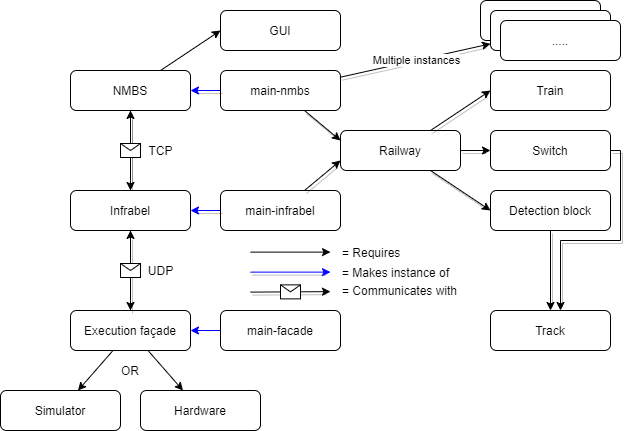
\includegraphics[width=\textwidth]{Images/software-architecture PP2.png}
        \caption{Afhankelijkheids diagram}
\end{figure}
\section{Beschrijving van API tussen infrabel- en NMBS-component}
\begin{table}[h!]
        \centering
        \begin{tabular}{|p{6.5cm}|p{6.5cm}|}
                \hline
                \multicolumn{1}{|>{\centering\arraybackslash}p{6.5cm}|}{\textbf{NMBS naar Infrabel}} 
                & \multicolumn{1}{>{\centering\arraybackslash}p{6.5cm}|}{\textbf{Infrabel terug naar NMBS}}\\
                \hline
                Vraagt informatie over de spoor objecten en locomotief objecten & Geeft lijsten van informatie over de spoor objeten en locomotief objecten terug.\\
                \hline
                Vraagt om de verbinding te sluiten & /\\
                \hline
                Vraagt om de stand van een wissel te veranderen & Stuurt de nieuwe stand van de wissel terug\\
                \hline
                Vraagt om de eindbestemming te zetten en het automatisch trajectbeheer in gang te steken & Vraagt een herberekening indien dit aangevraagd is terwijl de locomotief niet detecteerbaar is.\\
                \hline
                Vraagt om een locomotief to te voegen aan het spoornetwerk. & Geeft de gegevens van de toegevoegde locomotief terug om op de UI te kunnen zetten.\\
                \hline
                Vraagt om de richting van een locomotief te veranderen & Geeft de nieuwe richting terug. \\
                \hline
        \end{tabular}
\end{table}
\begin{table}[h!]
        \centering
        \begin{tabular}{|p{6.5cm}|p{6.5cm}|}   
                \hline
                Vraagt om de snelheid van een locomotief te wijzigen. & Geeft alleen de nieuwe snelheid terug indien deze nul is. \\
                \hline
                Vraagt om de het reservatieprotocol te wijzigen van een locomotief & /\\
                \hline
                Vraagt om een locomotief van het spoornetwerk te verwijderen & /\\
                \hline
                Vraagt om de simulator of hardware op een gegeven manier te starten & /\\
                \hline
       \end{tabular}
        \caption{Van NMBS naar Infrabel en terug}
\end{table}
\begin{table}[h!]
        \centering
        \begin{tabular}{|p{6.5cm}|p{6.5cm}|}
                \hline
                \multicolumn{1}{|>{\centering\arraybackslash}p{6.5cm}|}{\textbf{Infrabel naar NMBS}} 
                & \multicolumn{1}{>{\centering\arraybackslash}p{6.5cm}|}{\textbf{NMBS terug naar Infrabel}}\\
                \hline
                Stuurt logboek evenementen (verandering snelheid, richting etc.) & / \\
                \hline
                Stuurt berekende routes & /\\
                \hline
                Stuurt een lijst van de bezette spoorsegmenten & /\\
                \hline
                Stuurt een lijst van de gereserveerde spoorsegmenten & /\\
                \hline
        \end{tabular}
\end{table}
\section{Planning}
\begin{table}[h!]
        \centering
        \begin{tabular}{|p{2cm}|p{11cm}|}
                \hline
                \multicolumn{1}{|>{\centering\arraybackslash}p{2cm}|}{\textbf{Week}} 
                & \multicolumn{1}{>{\centering\arraybackslash}p{11cm}|}{\textbf{Gepland}}\\
                \hline
                5 & 18/10 Indienen voorstudie. \\
                \hline
                6 & Stuurt berekende routes \& Feedback afwachten, ADT detectieblok en switch implementeren.\\
                \hline
                7 & ADT locomotive \& track implementeren.\\
                \hline
                8 & ADT railway \& beginnen aan ADT infrabel.\\
                \hline
                9 & ADT infrabel \& NMBS component maken.\\
                \hline
                10 & Laatste aanpassingen NMBS.\\
                \hline
                11 & 18/10 Indienen fase 1: code en documentatie.\\
                \hline
                12 & Feedback afwachten.\\
                \hline
                13 \& 14 & Implementeren van grafen voor het automatisch trajectbeheer.\\
                \hline
                15 \& 16 & Automatisch trajectbeheer implementeren.\\
                \hline
                17 & Mogelijk maken dat GUI het traject kan tonen aan de hand van het trajectbeheer.\\
                \hline
                18 \& 19 & Botsingen voorkomen implementeren.\\
                \hline
                20 & GUI aanpassingen voor mogelijk extra componenten.\\
                \hline
                21 & Feedback vragen.\\
                \hline
                22 + 23 + 24 + 25 & Aanpassingen doorvoeren aan de hand van de feedback.\\
                \hline
                26 & 14/03 Indienen fase 2: code en documentatie.\\
                \hline
                27 & Feedback afwachten.\\
                \hline
        \end{tabular}
\end{table}
\begin{table}[h!]
        \centering
        \begin{tabular}{|p{2cm}|p{11cm}|}
                \hline
                28 + 29 + 30 + 31 & RPI.\\
                \hline
                32 & GUI aanpassen indien nodig.\\
                \hline
                33 + 34 + 35 & Hardware film maken/aanpassingen doorvoeren indien nodig.\\
                \hline
                36 & 23/05 Indienen fase 3: code en documentatie.\\
                \hline
        \end{tabular}
        \caption{Planning}
\end{table}
\section{Logboek}
\begin{table}[h!]
        \centering
        \begin{tabular}{|p{2cm}|p{11cm}|}
                \hline
                \multicolumn{1}{|>{\centering\arraybackslash}p{2cm}|}{\textbf{Week}} 
                & \multicolumn{1}{>{\centering\arraybackslash}p{11cm}|}{\textbf{Gepland}}\\
                \hline
                5 & 18/10 Ingediend voorstudie.\\
                \hline
                7 & ADT locomotive \& track implementeren.\\
                \hline
                8 & ADT railway \& beginnen aan ADT infrabel.\\
                \hline
                9 & ADT infrabel \& NMBS component maken.\\
                \hline
                11 & Code en documentatie ingeleverd (fase 1).\\
                \hline
                24 & Aanpassingen detectieblok ADT, Track ADT, switch ADT.\\
                \hline
                25 & Aanpassingen Locomotive ADT, Infrabel ADT.\\
                \hline
                26 & Aanpassingen NMBS ADT, Implementeren reservatiesysteem en deel van TCP. Code en documentatie ingeleverd (fase 2).\\
                \hline
                29 & Powerpoint gemaakt en projectverdediging.\\
                \hline
                30 & Aanpassingen reservatiesysteem.\\
                \hline
                31 \& 32 & Aanpassingen reservatiesysteem, GUI en trajectbeheer\\
                \hline
                33 & Aanpassingen automatisch trajectbeheer en testen met RPI.\\
                \hline
                34 & Verslagen geschreven. \\
                \hline
                36 & code en documentatie ingeleverd (fase 3). \\
                \hline
        \end{tabular}
        \caption{Logboek}
\end{table}
\end{document}
 